\documentclass[tikz,border=6pt]{standalone}
\usepackage{pgfplots}
\pgfplotsset{compat=1.18}
\begin{document}
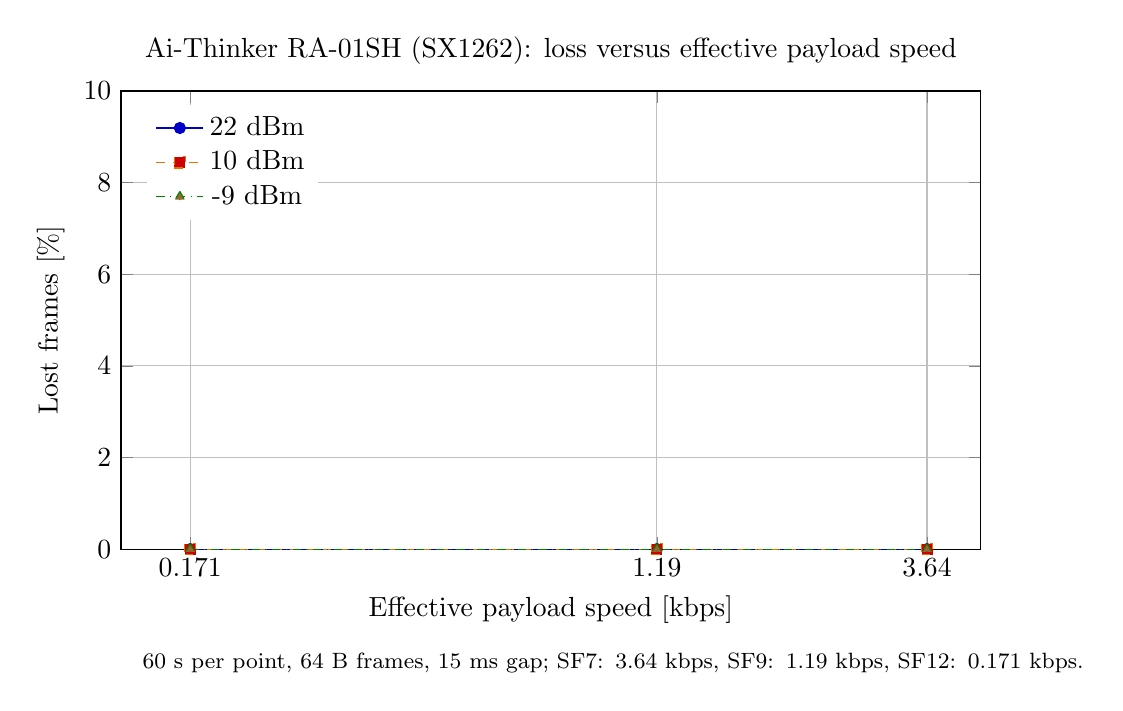
\begin{tikzpicture}
\begin{axis}[width=12.5cm,height=7.4cm,
 title={Ai-Thinker RA-01SH (SX1262): loss versus effective payload speed},xmode=log,xmin=0.128,xmax=4.55466667,ymin=0,ymax=10,
 xtick={0.170666667,1.18613333,3.64373333},xticklabels={0.171,1.19,3.64},
 xlabel={Effective payload speed [kbps]},ylabel={Lost frames [\%]},grid=both,legend style={draw=none,at={(0.03,0.97)},anchor=north west}]
\addplot+[blue!75!black,solid,mark=*] coordinates {(0.170666667,0) (1.18613333,0) (3.64373333,0)};
\addlegendentry{22 dBm}
\addplot+[orange!90!black,dashed,mark=square*] coordinates {(0.170666667,0) (1.18613333,0) (3.64373333,0)};
\addlegendentry{10 dBm}
\addplot+[green!50!black,dashdotted,mark=triangle*] coordinates {(0.170666667,0) (1.18613333,0) (3.64373333,0)};
\addlegendentry{-9 dBm}
\end{axis}
\node[font=\footnotesize,align=center,text width=12cm] at (6.25,-1.45) {60 s per point, 64 B frames, 15 ms gap; SF7: 3.64 kbps, SF9: 1.19 kbps, SF12: 0.171 kbps.};
\end{tikzpicture}
\end{document}
